\documentclass[conference]{IEEEtran}
\IEEEoverridecommandlockouts
% The preceding line is only needed to identify funding in the first footnote. If that is unneeded, please comment it out.
\usepackage{cite}
\usepackage{amsmath,amssymb,amsfonts}
\usepackage{algorithmic}
\usepackage{graphicx}
\usepackage{textcomp}
\usepackage{xcolor}
\def\BibTeX{{\rm B\kern-.05em{\sc i\kern-.025em b}\kern-.08em
    T\kern-.1667em\lower.7ex\hbox{E}\kern-.125emX}}
\begin{document}

\title{Addressing Crash Recovery With Persistent Memory Allocation\\
{\footnotesize \textsuperscript{}}
}

\author{\IEEEauthorblockN{\textsuperscript{} Nicholas Stone}
\IEEEauthorblockA{\textit{Xavier University} \\
Cincinnati Ohio, USA \\
Stonen2@Xavier.edu}

}
\maketitle

\begin{abstract}
Persistent memory is a combination of both volatile memory and long-term storage.  This means Persistent memory is able to maintain the speed of volatile memory such as Dynamic Random-Access Memory (DRAM) and is like the long-term storage of devices such as Solid-State Drive (SSD) and Hard Disk Drive (HDD), in its ability to maintain its state without consuming power. Furthermore, since persistent memory has Byte addressability and long-term storage, allocators can be used to maintain Data-structures that will persist even after power failure or program crashes. While persistent memory has unique characteristics that DRAM does not have, persistent memory has a few draw backs. Excessive writes to a single memory cell can destroy it and writes on persistent memory are much slower than reads. In this project we will be creating a memory allocator that will leverage both DRAM and Non-Volatile Random-Access Memory (NVRAM) to perform smart memory allocation that will be able to allow a data structure’s integrity to be preserved despite crashes and power failures without excessive writing to the persistent memory.
\end{abstract}

\begin{IEEEkeywords}
HDD,SSD,allocator,NVRAM,Persistent Memory
\end{IEEEkeywords}

\section{Introduction}
Non-Volatile Random-Access Memory (NVRAM) is a new kind of persistent memory that has a few unique characteristics that are different than that of Random-Access Memory (RAM).  The first is that this new form of technology allows for byte addressable long-term storage means that operate and execute several orders of magnitude faster than that of both Hard Disk Drives (HDD) and Solid-State Drives (SSD). Another unique factor of NVRAM is that this form of technology has a limited number of writes before the memory cells becomes unusable. If a program is not implemented properly or poorly the program can destroy memory cells rapidly thus damaging the technology and rendering it more expensive to use than typical RAM. One of the underlying tools that a programmer does not need to worry about usually is the allocator that a program is running or using.  Meaning that if a programmer was to write a program that was constantly writing to the same memory cells this could lead to a short life span of the NVRAM technology. It then becomes critical the smart memory allocations and tactical memory writes is used to leverage the NVRAM technology to be most effective. 
\\
Memory allocators have been used in systems since the early 1960s with the buddy memory allocation being implemented and used in 1963. As described above NVRAM has some unique properties that will enhance the runtime and performance of programs. However, if the same memory allocators that are used for RAM are used for NVRAM a large performance increase might not be experienced since these tactics are designed to run efficiently on RAM. The Memory allocating tactics that are used in this paper and program inherit some of the same or similar tactics to those that run on RAM but have a few unique characteristics that make them different. The first is that while locality is important for RAM technologies locality is critical for NVRAM technologies. Since NVRAM allows for data to persist even when a power cycle happens this means that any data in memory will be preserved on start up. Thus, allowing for a second program or an allocator to go through and find and restore all data that a program would have been using before a power cycle.  If a program can execute a systematic approach to memory allocation, then a simple algorithm can be implemented to then restore data in a quick and efficient manner. The second thing is that custom memory allocators may become more beneficial on NVRAM technologies than that of RAM \cite{berger-oopsla-2002 \cite{berger-oopsla-2009}}. This is due to the fact that NVRAM could be leveraged in a variety of ways by many different systems, meaning that a DMBS might use NVRAM to hold ‘Hot’ Tuples while a Cloud system might use allocation tactics differently.  The following memory allocator aims to see what kind of allocation tactics yields the best performance for programs while utilizing both RAM and NVRAM technologies. 


\section{Background}
The following section will explain the two main components that this paper focuses on, NVRAM and memory allocation. The following will not go into detail about the algorithms or tactics that the memory allocation in this paper will use, those details will be explained in further detail later on in this paper. 
\subsection{Persistent Memory Non-Volatile Random Access Memory}
NVRAM is a new and emerging kind of persistent memory that acts very similarly to RAM but also has a few key differences. The major differences are that this form of memory allows for byte addressability and has a much faster write time than that of both Hard Disk Drives (HDD) and Solid-State Drives (SSD). This order of magnitude is also followed by similar read times as that of RAM. Continuing from this NVRAM has the ability for data being stored to have long term storage like that of HDD or SSD when a power cycle occurs. One of the main drawbacks of NVRAM is that the memory has a write endurance, meaning that if too many write occur in a given memory cell that memory cell can be destroyed and no longer used. Obviously when memory cells are destroyed more writes will occur over more memory cells causing the destruction of NVRAM to happen quickly. NVRAM is not going to be replacing RAM in this allocation tactic but will be used alongside RAM. By leveraging both technologies we hope to allow preservation of data as well as long term use of the NVRAM technology.
\subsection{Memory Allocation}
A memory allocator is a program that is responsible for maintaining and distributing memory to be used by other programs. Part of the maintaining process is to make sure that all memory is distributed with the goal of locality as well as making sure that memory is returned to the operating system once the program no longer needs it. In this paper the main memory allocation tactic used is arena allocation, or the method of sectioning off large chunks of memory and then further distributing smaller sections of memory to be used by a program. By using this type of allocation, a second level of abstraction is added to the memory allocation and allows for arenas to maintain already allocated sections of memory while the allocator is able to distribute more arenas to a program. This allows for concurrency to flow in a program and can help stop bottle necks from occurring. This form of dynamic memory allocation is only one of many and used arenas in all of the data structures that will be listed here after. 


\section{Related Work}
While Persistent memory is a new and emerging technology the following related works that will be listed here after all pertain to persistent memory or memory allocation. While each of the papers uses and performs different kinds of memory allocation tactics it is important to highlight that these papers all use different approaches. The first related work we highlight is going to be Hoard which is a scalable memory allocator for multithreaded applications. It is important that we highlight that Hoard was able to accomplish four very important aspects if memory allocator performance. These four aspects are scalable, speed, false sharing avoidance, low fragmentation. It is important to note that the allocator that we are building is going to aim to achieve all of the following things however some of these things may suffer since we are building it for persistent memory. A second related work is Makalu a fast-recoverable allocation for non-volatile memory. It is important to note that once again this paper was able to highlight four very important aspects of fast recovery. These four things are failure induced inconsistencies, Transient versus persistent meta data, online failure consistency overhead vs recovery, and safe deallocation. Amongst these tactics we will focus mainly on safe deallocation tactics to be used by NVRAM. The last related work that we are going to highlight is going to be How to Build a Non-Volatile memory database management system. While this related work is rather short it does give an insight into some of the tactics that could be used if one was going to build a DBMS on top of NVRAM technologies. The main goal being how to utilize the technology to take in as few number of writes as possible while executing large amount of reads on the technology. This is done through placing ‘Hot’ Tuple in the NVRAM technology. 
\section{Visualization of Data-Structure} 
As discussed previously in this paper the goal of the NVRAM allocator is to make sure that locality is key, or the goal is making sure all data structures are placed in memory in some form of sequential chain. This allows a program to very quickly traverse the data structures and then allocate memory to the programmer. Here after will show the transformation in the data structure and show the improvement in locality as well as use of the free list algorithm. 
\subsection{Iteration 1}
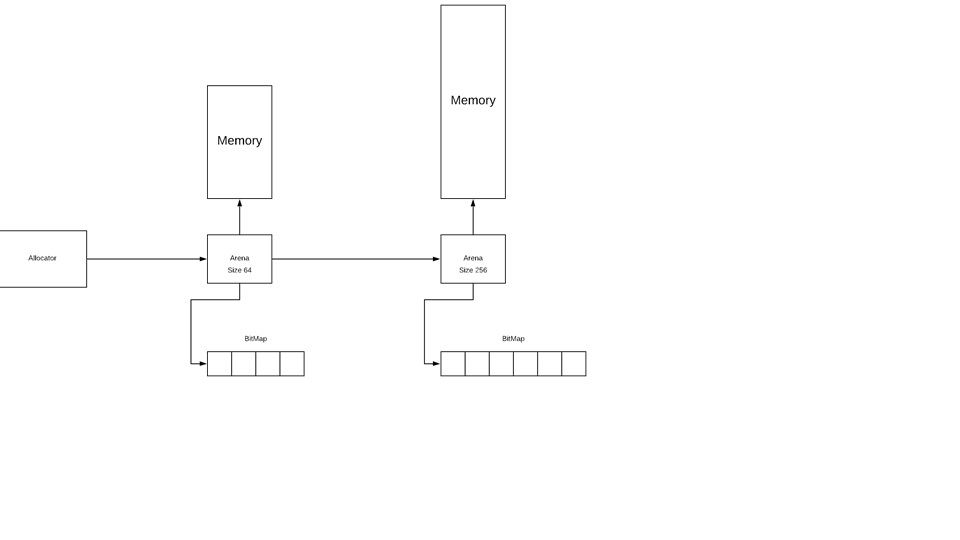
\includegraphics[width=14cm]{iteration1datastructure.jpg}
\caption{First Iteration of the Arena Data Structure}
\label{fig1:Iteration1}
The first iteration focuses mainly on making and connecting the bitmap data structure to map to an overall section of memory. This meaning that one bit in the bitmap correlates to a number of bits and that when the bit is 0 then the memory can be allocated and if the bit is 1 then the memory is already allocated. This then allows for a single list for the program to iterate through and check each bit map for an opening to allocate memory from. This meaning that threads could all loop through this one list and then check each arena if there is room to be allocated. Two main lessons were learned in this iteration, that concurrency suffers when only one free list is used. The second lesson is the locality of this data structure is very weak. That is that the array may not always be close in memory to the given arena that the bit map belongs too. 


\subsection{Iteration 2} 
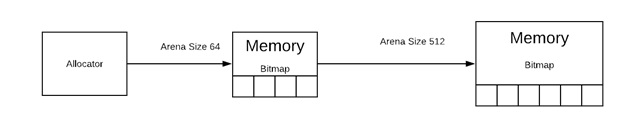
\includegraphics[width=8cm]{Iteration2datastructure.jpg}
\caption{Second Iteration of the Arena Data Structure}
\label{fig2:Iteration2}
The second iteration aimed to fix the locality problem that the first iteration experienced. By putting the bitmap inside the arena, we have increased the locality of each given arena allowing for easier recovery and allocation tactics. The key thing in this iteration is that there is still only one list, and this can form a bottle neck when it comes to concurrency. The same allocation tactic is used in both iteration 1 and iteration 2 and was described in iteration 1. 



\subsection{Iteration 3}
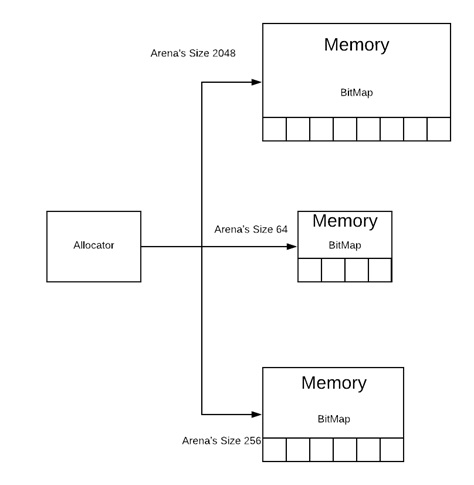
\includegraphics[width=8cm]{Iteration3datastructure.jpg}
\caption{Third Iteration of the Arena Data Structure}
\label{fig3:Iteration3}
From the figure listed you can see that the locality improvement from iteration 2 is preserved as well as multiple free lists have been implemented. This is largely due to a critical change in the allocation tactic, the rest of this paragraph aims to explain the new allocation tactic. The allocator will take in a given size that needs to be allocated by the program. The program then rounds that number up to a preset value, usually a factor of 64. Once this has been rounded the allocator will then search the list that contains all arenas with the value of the new rounded size. If that list is empty then a new arena will be created and added to the list, however if a new node is already being created then the program will allocate memory from a arena from the next list whose size is greater than that of the padded value. Once a value get above 4096 or above 1 page then the list contains all arenas whose value is greater than 4096. 

\subsection{Algorithms Explained}
The Following section will explain the algorithms in every level of abstraction in the persistent memory arena allocator. Recall from the previous sections of this paper that our allocator consists of two main components of functionality for memory management. The lowest level of abstraction is the arena level of the allocator. The functionality of this level is to perform and create a data structure to operate and maintain the arena level of the allocation. This means that this level of the allocator for our allocator is the level that will hold the bitmap as well as several other non-important pieces of metadata that allow for a list data structure to be created. Once again, the goal of this level of the allocator is to allow the overall program to keep creating and sectioning off arenas while the arenas are able to individually allocate memory to a program. This means that a programmer might want to allocate several 4-byte sized data types in the program. By allowing arenas to perform this action then you can stop bottlenecks from forming and allow for more operations to get done concurrently. The algorithm for the arena level is that as of iteration 1 each bit in the bit map can map to 1 byte of data. The arena is responsible for searching the list and then making sure that there is enough room for a data object of the size given can be allocated in a given arena. This is also responsible for returning what the location of where the object will be stored will go. The free functions take in an arena and then sets all of the bits in the bit maps and resets them to be 0 or in the state that they are ready to be allocated. The arena allocating level is only responsible for traversing free lists or lists of arenas and then calling the arenas to create and add a new arena to a free list.  

\section{Problems}
As mentioned above the NVRAM has both pros and cons and while the pros can be used to increase performance in programs the cons can lead to devastating impacts in the long term for a program. For example, if the creation of an allocator that only leverages NVRAM technologies might have an immediate increase in runtimes the lifetime of the NVRAM will be minimal as well as current RAM allocating tactics will not utilize NVRAM to is full potential. New allocating tactics should be examined since locality of memory in for NVRAM is critical as well as using both RAM and NVRAM in order to make a reliable and fast allocator becomes the main goal. The biggest problem then becomes understanding which of the many allocating tactics would be most efficient on this new technology. 
\section{Implementation Problems}
Before undertaking this project, I had done minimal systems work and even less work pertaining to memory allocators and changing the way that memory is allocated in a program beyond New and delete. The first of the many implementation problems that occurred was understanding the data structures and how they work together to achieve an efficient means to allocate memory. The implementation problem then occurred with linking the idea of an arena and how each arena needs to store a data structure or bit map to be able to track which parts of the memory have been allocated. The next implementation obstacle was building data structures and the level of abstraction for arena’s that allow for strong locality. Meaning that all of the data is being stored in or near one another. The last implementation problem that I will highlight in this paper is understanding which memory preservation tactic would work best and most efficient at the same time. With the instruction of placement new it became difficult to write reliable algorithms using placement new without overwriting nodes that are still in use.  
\section{Implementation Solutions}
In systems the greatest implementation solution that I have found to help solve all of my problems is to start with a picture. Meaning that when implementation problems occurred such as not fully understanding how the bitmap would interact with the arena data structures once a picture was drawn further ideas and tactics could be understood and then implemented. Not all of the ideas that are gathered from a picture work or are efficient, but it was a clear way of understanding the data structures. As for allocation tactics that would be used to reclaim memory with instructions such as placement new the tactic of free was to be changed to understand how much the free function will impact performance. Namely this meaning that free would not free any memory back to the OS but would reset an arena back to be completely cleared of all data and was ready to be used by the program. 



\section{API}
The following section will describe the API that belongs with the allocator that has been built thus far. This API aims to provide a simple interface for a programmer to interact with the allocator. It is important to note that this paper describes arenas and allocating tactics however a programmer will not need to know this information to use the API. These built in API calls will be utilizing the tactics listed above but are not necessary to use the API. 
\subsection{Init}
This function call initializes the allocator and MUST be called before the allocator can be used. This function is responsible for starting and initializing all of the free lists as well as takes in two parameters. The parameters are the location (Void *) of the region that is to be mapped and the second parameter is the size that has been allocated and is allowed to be used by the program. By providing these two parameters an initialized arena allocator will then be able to adequately implement arenas without going over the size that can be allocated by the program. When MMAP is implemented in this arena then this function will also be responsible for calling MMAP and placing the region given into virtual memory. 
\subsection{Destroy}
Currently this function is a No-Op or that this function has no operations. However, when MMAP is implemented this function will be responsible for using the munmap function to return the memory back to the operating system. This function takes in no parameters. 
\subsection{Get mem}
This function is responsible for doing most of the heavy lifting, namely this function is responsible for traversing the free lists and returning a location (Void*) to the programmer. This function will take in the size of an object that a programmer wants to allocate. Then it will pad this size and find the arena whose size is a factor of 64. If the list is currently empty, then the program will then create an arena of the new padded size. If a thread is already creating a new node then the allocator will search the next list with the next size above the padded size. Then the same steps if the list has space then allocate if not then we can create an arena. You will note that this kind of tactic is a lock free concurrency tactic. This will always yield a location that a programmer will get and allocate too. 
\subsection{Return mem}
This function will take in a pointer to a location a (void*) this function will then return the arena that this void * belongs too. This algorithm is actually trivial, since each arena has a start address and an end address then the program will check if the location given lies between the start and end locations of a given arena. If this location is within these bounds, then it will return this arena since it belongs in this arena other wise it will search the next arena or the next free list.
\section{Evaluation}
The following section will show the results of a series of tests run against the first iteration of the memory allocator against the Hoard memory allocator. The following tests look at the overall execution time of two different kind of test programs. Each of the test shows 5 runs averaging 10 successful execution of the test program. Once again it is important to recognize that these tests were run against the first iteration of the memory allocator. It is also important to note that these tests only look at the overall execution time of the program and are not looking at other aspects of performance. We expect our results to not be as efficient as the Hoard allocator and tactics on improving the iterations and what to change will be listed here after. The first test aims to show the average time and speed of the programs over a series of several small allocations. Recall that the Int data type has a size of 4 bytes and that a word has a size of 8 bytes. Thus, the first test allocates 10 Integers followed immediately by 15 Strings and then followed by another 15 Integers. The goal of the Arena allocation tactic is to limit the number of regions that are being mapped and trying to utilize sections of memory before allocating more chunks. Initially you can see that our memory allocator is only two orders of magnitude slower than that of the hoard allocator. Recall that an unsigned 64-bit pointer has a size of 8 bytes, the second test aims to focus on allocating larger sections of data instead of several smaller allocations. This allocation program was run with once again averaging 10 successful runs over 5 trials. In the case of both Hoard and our allocator we see that both of our programs experience a large performance increase in allocating medium sized sections of memory. In both trials we experience an increase in one order of magnitude.  



\begin{tabular}{ |p{1cm}||p{3cm}|p{3cm}|  }
 \hline
 \multicolumn{3}{|c|}{Test 1} \\
 \hline
 & Persistent Allocator & Hoard \\
 \hline
 Run 1   &3.4427909    &3.7682\\
 Run 2&   3.527523  & 4.8371   \\
 Run 3 &3.450038 & 3.7466  \\
 Run 4& 3.520118& 4.2558\\
 Run 5&   3.276502  &3.8146\\
 \hline
\end{tabular}
 The Following Tables Persistent Allocation is 10^-4 Seconds and Hoard is 10^-6
\\

\\
\\
\\

\\

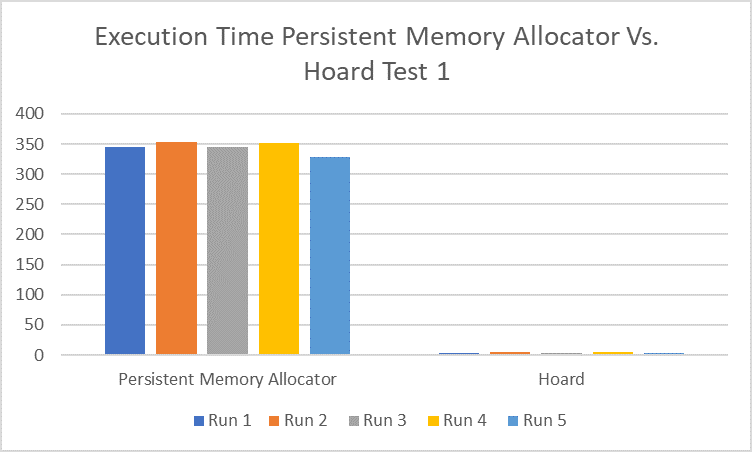
\includegraphics[width=8cm]{llllllllll.png}
\caption{Runtime results for Test 2 In Terms of Seconds * 10^-7}
\label{fig4:Test 1}
\\
\\


\begin{tabular}{ |p{1cm}||p{3cm}|p{3cm}|  }
 \hline
 \multicolumn{3}{|c|}{Test 2} \\
 \hline
 & Persistent Allocator & Hoard \\
 \hline
 Run 1   &9.64361    & 4.33\\
 Run 2& 9.54612    &  4.588  \\
 Run 3 &9.59781 &  4.403 \\
 Run 4&9.55489 & 4.566\\
 Run 5&  9.54126  & 4.279\\
 \hline
\end{tabular}
 The Following Tables Persistent Allocation is 10^-5 Seconds and Hoard is 10^-7
\\
\\

\\

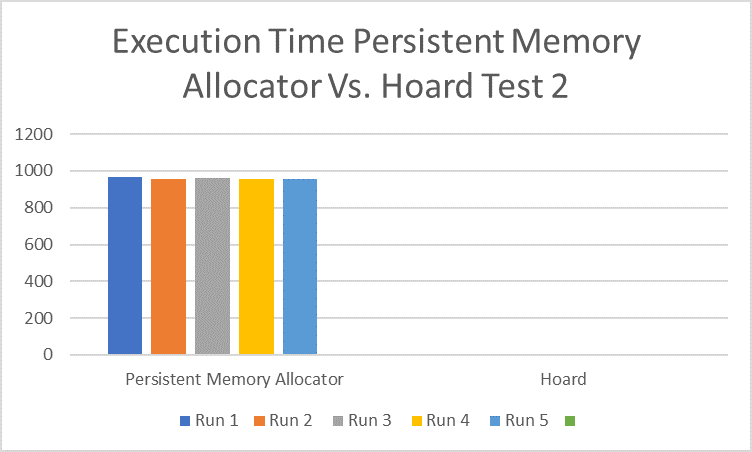
\includegraphics[width=8cm]{lll.png}
\caption{Runtime results for Test 2 In Terms of Seconds * 10^-7}
\label{fig5:Test 2}
\\

\\
Further optimizations were implemented in iteration 1 in order to re-run test and improve latency performance
\\
\\

\begin{tabular}{ |p{1cm}||p{3cm}|p{3cm}|  }
 \hline
 \multicolumn{3}{|c|}{Test 1 Optimization has Occurred} \\
 \hline
 & Persistent Allocator & Hoard \\
 \hline
 Run 1   &1.787    & 3.7682\\
 Run 2& 1.79267    &   4.8371  \\
 Run 3 &1.7953 &  3.7466 \\
 Run 4&1.787834& 4.2558\\
 Run 5& 1.794834  & 3.8146\\
 \hline
\end{tabular}
 The Following Tables Persistent Allocation is 10^-5 Seconds and Hoard is 10^-6\\
 
 \\
 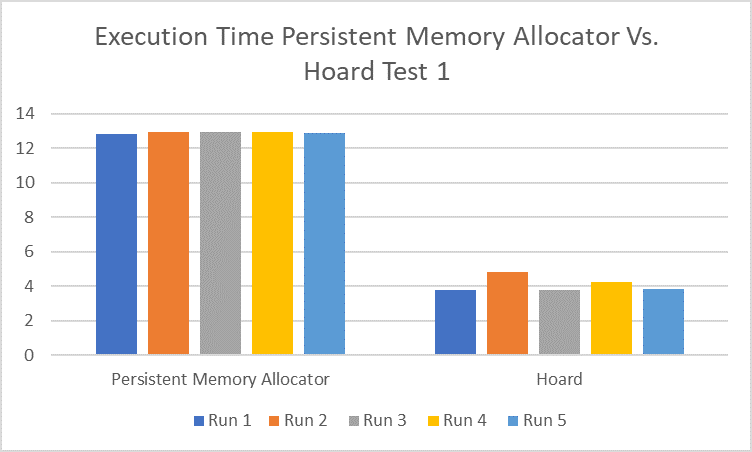
\includegraphics[width=8cm]{Hoardgraph1.png}
\caption{Runtime results for Test 1 In Terms of Seconds * 10^-6 Optimized}
\label{fig6:Test 1 Optimized}
\\
 

\begin{tabular}{ |p{1cm}||p{3cm}|p{3cm}|  }
 \hline
 \multicolumn{3}{|c|}{Test 2 Optimization has Occurred} \\
 \hline
 & Persistent Allocator & Hoard \\
 \hline
 Run 1   &4.2186    & 4.33\\
 Run 2& 4.2324    &  4.588  \\
 Run 3 &4.155 &  4.403 \\
 Run 4&4.1953& 4.566\\
 Run 5& 4.2827  & 4.279\\
 \hline
\end{tabular}

The Following Tables Persistent Allocation is 10^-6 Seconds and Hoard is 10^-7\\

 \\
 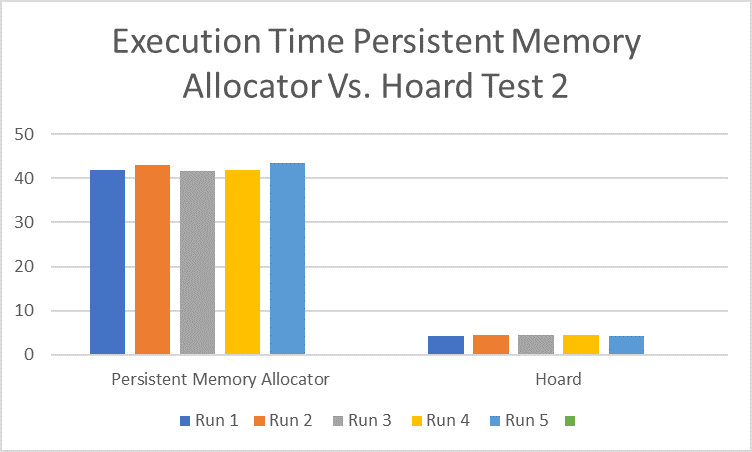
\includegraphics[width=8cm]{HoardGraph2.png}
\caption{Runtime results for Test 2 In Terms of Seconds * 10^-7 Optimized}
\label{fig7:Test 2 Optimized}
\\
 

\newline

As described in other sections of this paper the reason for such a drastic performance increase starts in the overall design of our data structure. This meaning that while locality could explain a minor decrease in performance the major reason for such a slow down is in the amount of memory that each arena is allocating in our memory allocator. Recall that iteration 1 of our allocator started by making sure each node in the list that was created was twice the size of the previous Arena and that the starting Arena size is 64 bytes. Furthermore, before another arena is to be allocated it must traverse the entire byte length of the arena before it. When string sizes are allocated there is a lot of wasted cycles and time being spent searching nodes that are completely full or have no room for allocating such sizes. Continuing from this there was no implementation for remember where the next best fit would be in each of the given arenas. Overall while the experiments run was trivial it still allows us some key insights in the flaws of our memory allocators but also in possible tactics to implement in the future. 
\section{Future Work}
The project currently provides a strong base and API that replicates and allows programmers to use an allocator that implements a form of smart allocating tactics. However, since NVRAM is a relatively new form of technology there are very few other kinds of NVRAM aware allocators. Thus, it would be unfair to compare speeds of NVRAM technologies against RAM technologies since as described above the technologies are different. From this future work on this project and allocator Is to implement at least two other kinds of allocators and compare these speeds against one another as well as RAM technologies. Along with these implementations the need for investigation in which concurrency tactic should be implemented. While ideally atomic operations should be utilized experiments of other kinds of concurrency tactics should be used in order to give programmers ideas of which method would be best for implementation of custom allocators. Mainly the goal of this second part is to share information of is the performance increase of atomic operations worth the time it takes to implement atomic allocations versus that of a spin lock allocation tactic. 

\section{Future Experiments}
It is important that experiments for all of the allocators that are tested, are executed on the basis of not only runtime performance but as well as concurrency and crash recovery. Namely that allocation times such as malloc and free should be tested but also the amount of time that each thread takes as well as the overall recovery time needs to be examined. That is if an arena allocator has poor free time, but recovery time is much faster that that of another form of dynamic memory allocation then use cases need to be examined before one type of allocator can be favored on NVRAM. Furthermore, the investigation of allocator data structures should also be examined, allowing a programmer to identify which type of data structure allows for fastest runtime. This means examining a free list tactic versus best fit tactic or a combination of both. 
\\
Future experiments need to be carefully thought about in advance before they must be run. As described above there is also an understanding in a trade off of performance to allow for memory allocators to operate on NVRAM. The following experiments that will be used will be broken off into more sections than just allocating alone. Furthermore, the allocating tactics will be broken into several groups other than just small allocations and medium sized allocations. Allocations will be broken into several tests and will be testing the ability to allocate large chunks of data as well as smaller chunks in random intervals. By doing this the test will replicate a real implementation as well as will ensure that allocators are not just optimized under the scenario that all data will be uniform. Continuing from these tests the individual allocators ability to free data will also be tested. 

\section{Conclusion}
Moving forward, this project is going to be focusing mainly on allocation tactics and learning and improving the performance with each iteration and change in the overall design of the allocator. Currently moving forward the overall data structure is strong and allows for fast performance inside each arena. It is also important to highlight and focus on every level of abstraction within this project. Thus, meaning that a focus needs to be on the design and execution of the allocator in the high level of ensuring that allocation techniques are correct but also ensuring that the arenas are operating and being allocated in a fast and efficient fashion. While our first experiment yielded results that show’s the strength of the Hoard allocator it was still able to give some keen insight on how the allocator operating can change. With every change the allocator can become more efficient, but an emphasis is also going to be placed around the new technology that this is being implemented for meaning that we will not forget about the constraint of NVRAM in order to gain speed. Careful consideration will still be placed on what is being written to persistent memory and what will be designated to RAM. Along with the consideration of performance, concurrency will be continued to be explored allowing our allocator to support multi-threading on NVRAM technology. Every test here after will be focused on examining the allocator in a way to continue to allow the team to enhance and better the data structures and algorithms used. 

\section{Acknowledgment}

I want to thank Lehigh University and the NSF for the opportunity to research memory allocation on the new and emerging technology NVRAM.  




\bibliographystyle{./bibliography/IEEEtran}
\bibliography{g.bib}

\vspace{12pt}






\end{document}

